% !TEX encoding = UTF-8
% !TEX TS-program = pdflatex
% !TEX root = ../tesi.tex

%**************************************************************
\chapter{Conclusioni}
\label{cap:conclusioni}
%**************************************************************

%**************************************************************
\section{Consuntivo}
Questa sezione descrive i risultati dello stage sotto forma di metriche. Nel complesso, il progetto si è concluso positivamente.

\subsection{Requisiti} %%%%%%%%%%%%%%%%%%%%%%%%%%%%%%%%%%
\textbf{Risultato: Passato}\\
L'applicazione soddisfa tutti i requisiti obbligatori (funzionali e vincolo)\riferimento{tab:requisiti-funzionali} (19/19) e metà dei requisiti desiderabili (2/4). I requisiti desiderabili non implementati, per questioni di tempo, sono RD-3 e RD-4\riferimento{tab:requisiti-funzionali-fine}, ovvero l'esposizione dell'applicazione attraverso un'API e la generazione delle informazioni di compilazione. Ho implementato questi requisiti in un breve periodo di post-stage in azienda.
\label{tab:requisiti-resoconto}
\begin{longtable}{|l l|}
\caption{requisiti soddisfatti}\\
\hline
\textbf{Requisito} & \textbf{Risultato} \\
\hline
\endhead
ROF-1     & soddisfatto\\
ROF-2     & soddisfatto\\
ROF-3     & soddisfatto\\
ROF-3.1   & soddisfatto\\
ROF-3.2   & soddisfatto\\
ROF-3.3   & soddisfatto\\
ROF-3.4   & soddisfatto\\
ROF-4     & soddisfatto\\
ROF-4.1   & soddisfatto\\
ROF-4.2   & soddisfatto\\
ROF-4.3   & soddisfatto\\
ROF-4.4   & soddisfatto\\
ROF-4.5   & soddisfatto\\
ROF-5     & soddisfatto\\
RDF-1     & soddisfatto\\
RDF-2     & soddisfatto\\
RDF-3     & non soddisfatto\\
RDF-4     & non soddisfatto\\
ROV-1     & soddisfatto\\
ROV-2     & soddisfatto\\
ROV-3     & soddisfatto\\
ROV-4     & soddisfatto\\
\hline
\end{longtable}

Il seguente grafico rappresenta la relazione tra requisiti totali soddisfatti e requisiti non soddisfatti.
\begin{figure}[H]
    \centering
    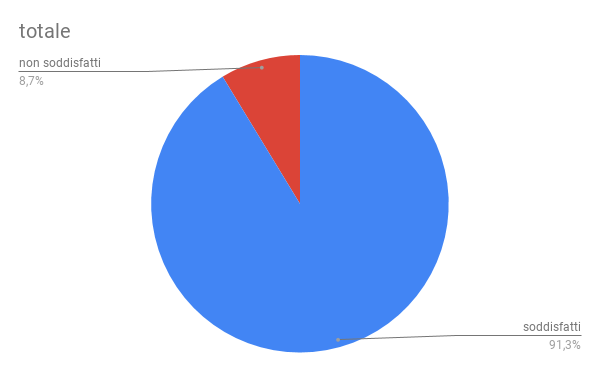
\includegraphics[width=0.8\textwidth]{results/req_total.png}
    \caption{Requisiti soddisfatti}
    \label{img:req_soddisfatti}
\end{figure}

Il seguente grafico rappresenta la relazione tra requisiti soddisfatti e non soddisfatti, separati per desiderabili e obbligatori.
\begin{figure}[H]
    \centering
    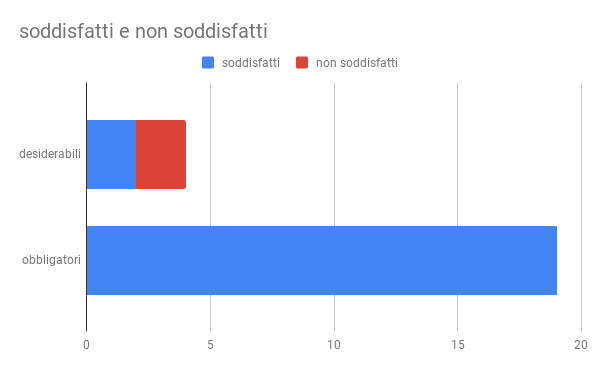
\includegraphics[width=0.8\textwidth]{results/req_sod.png}
    \caption{Requisiti totali}
    \label{img:req_totali}
\end{figure}

\subsection{Metriche del codice} %%%%%%%%%%%%%%%%%%%%%%%%%%%%%%
\subsubsection{Code coverage} %
\textbf{Risultato: Passato}\\
Il \textit{code coverage} è pari all'87\%, superiore dell'80\% richiesto dal requisito ROV-4\riferimento{tab:requisiti-vincolo}. I metodi non coperti sono molto semplici e non necessitano di essere testati.
\begin{figure}[H]
    \centering
    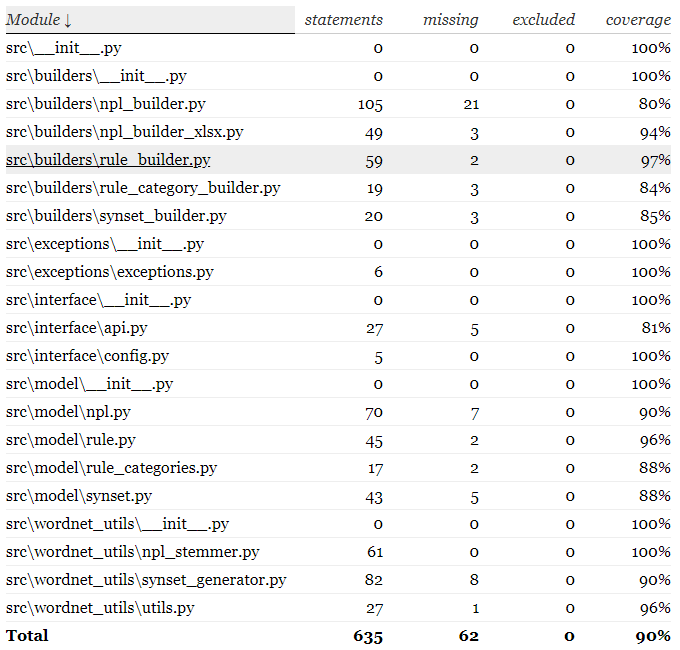
\includegraphics[width=0.9\columnwidth]{results/coverage.PNG} 
    \caption{code coverage}
    \label{coverage}
\end{figure}
\begin{figure}[H]
    \centering
    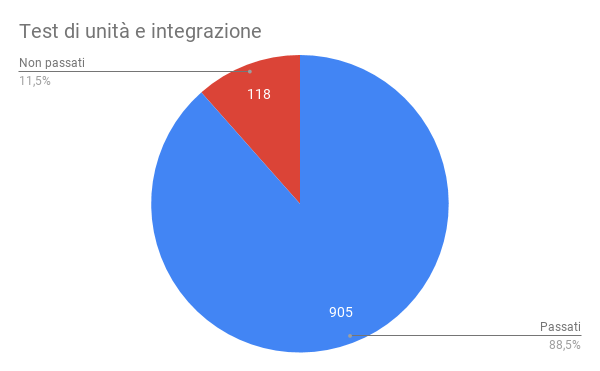
\includegraphics[width=0.8\columnwidth]{results/test_pie.png} 
    \caption{Test di unità e integrazione}
    \label{img:unittests}
\end{figure}

\subsubsection{Analisi statica} %
\textbf{Risultato: Passato}\\
Durante la codifica, ho utilizzato \textit{pycodestyle} per rispettare lo stile definito da PEP8, come da metrica ROV-5\riferimento{tab:requisiti-vincolo}. Questo ha portato a un codice privo di \textit{warning} da parte di \textit{pycodestyle}, relativi allo stile PEP8.
\begin{figure}[H]
    \centering
    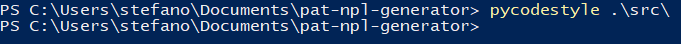
\includegraphics[width=0.9\columnwidth]{results/nostyle.PNG} 
    \caption{pycodestyle}
    \label{nosecov}
\end{figure}

\subsection{User satisfaction} %%%%%%%%%%%%%%%%%%%
\textbf{Risultato: Passato}\\
Questa metrica, seppure meno oggettiva delle precedenti, è basata sulla riunione tecnica tenuta con i ricercatori della Zucchetti S.R.L e il tutor aziendale.\\
L'incontro è avvenuto l'ultima settimana di stage, per capire come integrare {\app} alla loro applicazione. Attraverso dei diagrammi UML, ho spiegato il funzionamento degli algoritmi implementati.\\
La presentazione si è conclusa con successo. I ricercatori hanno capito come migliorare l'output della loro applicazione, fornito in input a {\app}.\\
Il tutor aziendale ha apprezzato particolarmente l'automatismo fornito da {\app}. Per questo motivo, ha deciso di integrarlo ad \textit{Engagent} attraverso una REST API.

%**************************************************************
\section{Raggiungimento degli obiettivi}

%**************************************************************
\section{Conoscenze acquisite}
\begin{itemize}
    \item gestione di un progetto in \textbf{python}, attraverso ambienti virtuali (per la gestione delle dipendenze) e principali librerie;
    \item importanza e il ruolo del \textit{pre-processing} dei dati, prima di essere elaborati da un algoritmo di machine learning. Nel mondo reale, i dati sono pochi e preziosi, quindi è necessario sfruttarli al massimo e assicurarsi che l'output dell'algoritmo di \textit{machine learning} sia filtrato e analizzato, prima di essere esposto agli utenti del servizio.\\ Questo si contrappone con l'esperienza universitaria, dove il focus principale viene posto sul metodo, invece che sul risultato.
    \item presentazione del software orientata a esperti (tecnica) e agli utenti (funzionale).
    \item ho potuto osservare nella pratica come funziona una \textit{software house} di piccole dimensioni, iniziando ad acquisire la professionalità richiesta per questo ambiente;
\end{itemize}
%**************************************************************
\section{Valutazione personale}
Prima di iniziare lo stage, sapevo che avrei voluto continuare il mio percorso di studi con la Laurea Magistrale, quindi ho considerato questa esperienza come un mezzo per imparare qualcosa di nuovo, invece di applicare banalmente quello che ho imparato negli anni.\\
Ho potuto, per la prima volta, partecipare a dei colloqui di lavoro, qualcosa di cui ho sempre avuto timore, ma che ho imparato a gestire fin da subito.\\
Lavorare in gruppo è sempre stato un mio limite, che ritengo di aver superato grazie ai progetti svolti durante l'ultimo anno di triennale e ovviamente con lo stage. Nella maggior parte delle situazioni, unire le conoscenze per svolgere un singolo compito può velocizzare considerevolmente il lavoro, soprattutto durante la codifica (ad esempio con il peer programming, attuato giornalmente durante il progetto di Ingegneria del Software, per le parti più delicate dell'applicazione) e durante l'analisi e progettazione del software (durante lo stage, le sessioni di brainstorming con i colleghi erano frequenti e hanno portato ottimi risultati).\\
Dopo la fine dello stage, ho svolto un periodo extra per portare il software in produzione, dato che erano soddisfatti del risultato. Durante questo periodo, ho imparato come generare automaticamente i \textit{log} durante l'esecuzione di un programma, quindi ho creato una REST API per renderlo disponibile alla rete aziendale. Questa esperienza di post-stage è qualcosa che non ho potuto sperimentare durante la laurea, ma essenziale in ambiente professionale.\\
Anche se non ho lavorato direttamente ad un algoritmo di machine learning, ho potuto capire la sua importanza nell'ambito professionale. Le aziende che investono (o intendono investire) in questa tecnologia sono portate ad acquisire sempre più dati dai propri clienti e/o partner, in quanto elemento fondamentale per un buon risultato. \company{} sta migliorando in questo compito, come molte altre aziende che vogliono rimanere competitive in un futuro poco lontano. Vedere quante risorse stanno investendo, mi ha motivato ancora di più a seguire un piano di studi orientato all'intelligenza artificiale: studierò qualcosa che mi piace, richiesto dal mercato e che acquisirà sempre più importanza in futuro.